% ------------------------------------------------------------------
\chapter{Computational blocks}\label{s:blocks}
% ------------------------------------------------------------------

This chapters describes the individual computational blocks supported by \matconvnet. The interface of a CNN computational block !<block>! is designed after the discussion in \cref{s:fundamentals}. The block is implemented as a MATLAB function !y = vl_nn<block>(x,w)! that takes as input MATLAB arrays !x! and !w! representing the input data and parameters and returns an array !y! as output. In general, !x! and !y! are 4D real arrays packing $N$ maps or images, as discussed above, whereas !w! may have an arbitrary shape.

The function implementing each block is capable of working in the backward direction as well, in order to compute derivatives. This is done by passing a third optional argument !dzdy! representing the derivative of the output of the network with respect to $\by$; in this case, the function returns the derivatives ![dzdx,dzdw] = vl_nn<block>(x,w,dzdy)! with respect to the input data and parameters. The arrays !dzdx!, !dzdy! and !dzdw! have the same dimensions of !x!, !y! and !w! respectively (see \cref{s:back}).

Different functions may use a slightly different syntax, as needed: many functions can take additional optional arguments, specified as property-value pairs; some do not have parameters  !w! (e.g. a rectified linear unit); others can take multiple inputs and parameters, in which case there may be more than one !x!, !w!, !dzdx!, !dzdy! or !dzdw!. See the rest of the chapter and MATLAB inline help for details on the syntax.\footnote{Other parts of the library will wrap these functions into objects with a perfectly uniform interface; however, the low-level functions aim at providing a straightforward and obvious interface even if this means differing slightly from block to block.}

The rest of the chapter describes the blocks implemented in \matconvnet, with a particular focus on their analytical definition. Refer instead to MATLAB inline help for further details on the syntax.

% ------------------------------------------------------------------
\section{Convolution}\label{s:convolution}
% ------------------------------------------------------------------

\begin{figure}[t]
	\centering
	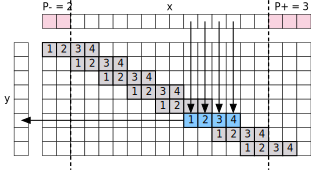
\includegraphics[width=0.7\textwidth]{figures/svg/conv}
	\caption{\textbf{Convolution.} The figure illustrates the process of filtering a 1D signal $\bx$ by a filter $f$ to obtain a signal $\by$. The filter has $H'=4$ elements and is applied with a stride of $S_h =2$ samples. The purple areas represented padding $P_-=2$ and $P_+=3$ which is zero-filled. Filters are applied in a sliding-window manner across the input signal. The samples of $\bx$ involved in the calculation of a sample of $\by$ are shown with arrow. Note that the rightmost sample of $\bx$  is never processed by any filter application due to the sampling step. While in this case the sample is in the padded region, this can happen also without padding.}\label{f:conv}
\end{figure}

The convolutional block is implemented by the function !vl_nnconv!. !y=vl_nnconv(x,f,b)! computes the convolution of the input map $\bx$ with a bank of $K$ multi-dimensional filters $\bff$ and biases $b$. Here
\[
 \bx\in\real^{H \times W \times D}, \quad
 \bff\in\real^{H' \times W' \times D \times D''}, \quad
 \by\in\real^{H'' \times W'' \times D''}.
\]
The process of convolving a signal is illustrated in \cref{f:conv} for a 1D slice. Formally, the output is given by
\[
y_{i''j''d''}
=
b_{d''}
+
\sum_{i'=1}^{H'}
\sum_{j'=1}^{W'}
\sum_{d'=1}^D
f_{i'j'd} \times x_{i''+i'-1,j''+j'-1,d',d''}.
\]
The call !vl_nnconv(x,f,[])! does not use the biases. Note that the function works with arbitrarily sized inputs and filters (as opposed to, for example, square images). See \cref{s:impl-convolution} for technical details.

\paragraph{Padding and stride.} !vl_nnconv! allows to specify  top-bottom-left-right paddings $(P_h^-,P_h^+,P_w^-,P_w^+)$ of the input array and subsampling strides $(S_h,S_w)$ of the output array:
\[
y_{i''j''d''}
=
b_{d''}
+
\sum_{i'=1}^{H'}
\sum_{j'=1}^{W'}
\sum_{d'=1}^D
f_{i'j'd} \times x_{S_h (i''-1)+i'-P_h^-, S_w(j''-1)+j' - P_w^-,d',d''}.
\]
In this expression, the array $\bx$ is implicitly extended with zeros as needed.

\paragraph{Output size.} !vl_nnconv! computes only the ``valid'' part of the convolution; i.e. it requires each application of a filter to be fully contained in the input support.  The size of the output is computed in \cref{s:receptive-simple-filters} and is given by:
\[
  H'' = 1 + \left\lfloor \frac{H - H' + P_h^- + P_h^+}{S_h} \right\rfloor.
\]
Note that the padded input must be at least as large as the filters: $H +P_h^- + P_h^+ \geq H'$, otherwise an error is thrown.

\paragraph{Receptive field size and geometric transformations.} Very often it is useful to geometrically relate the indexes of the various array to the input data (usually images) in terms of coordinate transformations and size of the receptive field (i.e. of the image region that affects an output). This is derived in \cref{s:receptive-simple-filters}.

\paragraph{Fully connected layers.} In other libraries, \emph{fully connected blocks or layers} are linear functions where each output dimension depends on all the input dimensions. \matconvnet does not distinguish between fully connected layers and convolutional blocks. Instead, the former is a special case of the latter obtained when the output map $\by$ has dimensions $W''=H''=1$. Internally, !vl_nnconv! handles this case more efficiently when possible.

\paragraph{Filter groups.} For additional flexibility, !vl_nnconv! allows to group channels of the input array $\bx$ and apply different subsets of filters to each group. To use this feature, specify as input a bank  of $D''$ filters $\bff\in\real^{H'\times W'\times D'\times D''}$ such that $D'$ divides the number of input dimensions $D$. These are treated as $g=D/D'$ filter groups; the first group is applied to dimensions $d=1,\dots,D'$ of the input $\bx$; the second group to dimensions $d=D'+1,\dots,2D'$ and so on. Note that the output is still an array $\by\in\real^{H''\times W''\times D''}$.

An application of grouping is implementing the Krizhevsky and Hinton network~\cite{krizhevsky12imagenet} which uses two such streams. Another application is sum pooling; in the latter case, one can specify $D$ groups of $D'=1$ dimensional filters identical filters of value 1 (however, this is considerably slower than calling the dedicated pooling function as given in \cref{s:pooling}).

\paragraph{Dilation.} !vl_nnconv! allows kernels to be spatially dilated on the fly by inserting zeros between elements. For instance, a dilation factor $d=2$ causes the 1D kernel $[f_1,f_2]$ to be implicitly transformed in the kernel $[f_1,0,0,f_2]$. Thus, with dilation factors $d_h,d_w$, a filter of size $(H_f,W_f)$ is equivalent to a filter of size:
\[
  H' = d_h(H_f - 1) + 1,
  \qquad
  W' = d_w(W_f - 1) + 1.
\]
With dilation, the convolution becomes:
\[
y_{i''j''d''}
=
b_{d''}
+
\sum_{i'=1}^{H_f}
\sum_{j'=1}^{W_f}
\sum_{d'=1}^D
f_{i'j'd} \times x_{
S_h (i''-1)+d_h(i'-1)-P_h^-+1,
S_w (j''-1)+d_w(j'-1)-P_w^-+1,
d',d''}.
\]


% ------------------------------------------------------------------
\section{Convolution transpose (deconvolution)}\label{s:convt}
% ------------------------------------------------------------------

\begin{figure}[t]
	\centering
	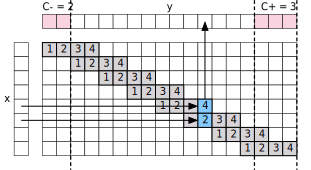
\includegraphics[width=0.7\textwidth]{figures/svg/convt}
	\caption{\textbf{Convolution transpose.} The figure illustrates the process of filtering a 1D signal $x$ by a filter $f$ to obtain a signal $y$. The filter is applied as a sliding-window, forming a pattern which is the transpose of the one of \cref{f:conv}. The filter has $H'=4$ samples in total, although each filter application uses two of them (blue squares) in a circulant manner. The purple areas represent crops with $C_-=2$ and $C_+=3$ which are discarded. The arrows exemplify which samples of $x$ are involved in the calculation of a particular sample of $y$. Note that, differently from the forward convolution \cref{f:conv}, there is no need to add padding to the input array; instead, the convolution transpose filters can be seen as being applied with maximum input padding (more would result in zero output values), and the latter can be reduced by cropping the output instead.}\label{f:convt}
\end{figure}

The \emph{convolution transpose} block (sometimes referred to as ``deconvolution'') is the transpose of the convolution block described in \cref{s:convolution}. In \matconvnet, convolution transpose is  implemented by the function !vl_nnconvt!.

In order to understand convolution transpose, let:
\[
 \bx\in\real^{H \times W \times D}, \quad
 \bff\in\real^{H' \times W' \times D \times D''}, \quad
 \by\in\real^{H'' \times W'' \times D''}, \quad
\]
be the input tensor, filters, and output tensors. Imagine operating in the reverse direction by using the filter bank $\bff$ to convolve the output $\by$ to obtain the input $\bx$, using the definitions given in~\cref{s:convolution} for the convolution operator; since convolution is linear, it can be expressed as a matrix $M$ such that  $\vv \bx = M \vv\by$; convolution transpose computes instead $\vv \by = M^\top \vv \bx$. This process is illustrated for a 1D slice in \cref{f:convt}.

There are two important applications of convolution transpose. The first one is the so called \emph{deconvolutional networks}~\cite{zeiler14visualizing} and other networks such as convolutional decoders that use the transpose of a convolution. The second one is implementing data interpolation. In fact, as the convolution block supports input padding and output downsampling, the convolution transpose block supports input upsampling and output cropping.

Convolution transpose can be expressed in closed form in the following rather unwieldy expression (derived in \cref{s:impl-convolution-transpose}):
\begin{multline}\label{e:convt}
y_{i''j''d''} =
 \sum_{d'=1}^{D}
 \sum_{i'=0}^{q(H',S_h)}
 \sum_{j'=0}^{q(W',S_w)}
f_{
1+ S_hi' + m(i''+ P_h^-, S_h),\ %
1+ S_wj' + m(j''+ P_w^-, S_w),\ %
d'',
d'
}
\times \\
x_{
1 - i' + q(i''+P_h^-,S_h),\ %
1 - j' + q(j''+P_w^-,S_w),\ %
d'
}
\end{multline}
where
\[
m(k,S) = (k - 1) \bmod S,
\qquad
q(k,n) = \left\lfloor \frac{k-1}{S} \right\rfloor,
\]
$(S_h,S_w)$ are the vertical and horizontal \emph{input upsampling factors},  $(P_h^-,P_h^+,P_h^-,P_h^+)$ the \emph{output crops}, and $\bx$ and $\bff$ are zero-padded as needed in the calculation. Note also that filter $k$ is stored as a slice $\bff_{:,:,k,:}$ of the 4D tensor $\bff$.

The height of the output array $\by$ is given by
\[
  H'' = S_h (H - 1) + H' -P^-_h - P^+_h.
\]
A similar formula holds true for the width. These formulas are derived in \cref{s:receptive-convolution-transpose} along with an expression for the receptive field of the operator.

We now illustrate the action of convolution transpose in an example (see also \cref{f:convt}).  Consider a 1D slice in the vertical direction, assume that the crop parameters are zero, and that $S_h>1$. Consider the output sample $y_{i''}$ where the index $i''$ is chosen such that $S_h$ divides $i''-1$; according to~\eqref{e:convt}, this sample is obtained as a weighted summation of $x_{i'' / S_h},x_{i''/S_h-1},...$ (note that the order is reversed). The weights are the filter elements $f_1$, $f_{S_h}$,$f_{2S_h},\dots$ subsampled with a step of $S_h$. Now consider computing the element $y_{i''+1}$; due to the rounding in the quotient operation $q(i'',S_h)$, this output sample is obtained as a weighted combination of the same elements of the input $x$ that were used to compute $y_{i''}$; however, the filter weights are now shifted by one place to the right: $f_2$, $f_{S_h+1}$,$f_{2S_h+1}$, $\dots$. The same is true for $i''+2, i'' + 3,\dots$ until we hit $i'' + S_h$. Here the cycle restarts after shifting $\bx$ to the right by one place. Effectively, convolution transpose works as an \emph{interpolating filter}.

% ------------------------------------------------------------------
\section{Spatial pooling}\label{s:pooling}
% ------------------------------------------------------------------

!vl_nnpool! implements max and sum pooling. The \emph{max pooling} operator computes the maximum response of each feature channel in a $H' \times W'$ patch
\[
y_{i''j''d} = \max_{1\leq i' \leq H', 1 \leq j' \leq W'} x_{i''+i'-1,j''+j'-1,d}.
\]
resulting in an output of size $\by\in\real^{H''\times W'' \times D}$, similar to the convolution operator of \cref{s:convolution}. Sum-pooling computes the average of the values instead:
\[
y_{i''j''d} = \frac{1}{W'H'}
\sum_{1\leq i' \leq H', 1 \leq j' \leq W'} x_{i''+i'-1,j''+j'-1,d}.
\]
Detailed calculation of the derivatives is provided in \cref{s:impl-pooling}.

\paragraph{Padding and stride.} Similar to the convolution operator of \cref{s:convolution}, !vl_nnpool! supports padding the input; however, the effect is different from padding in the convolutional block as pooling regions straddling the image boundaries are cropped. For max pooling, this is equivalent to extending the input data with $-\infty$; for sum pooling, this is similar to padding with zeros, but the normalization factor at the boundaries is smaller to account for the smaller integration area.

% ------------------------------------------------------------------
\section{Activation functions}\label{s:activation}
% ------------------------------------------------------------------

\matconvnet supports the following activation functions:
%
\begin{itemize}
\item \emph{ReLU.} !vl_nnrelu! computes the \emph{Rectified Linear Unit} (ReLU):
\[
 y_{ijd} = \max\{0, x_{ijd}\}.
\]

\item \emph{Sigmoid.} !vl_nnsigmoid! computes the \emph{sigmoid}:
\[
 y_{ijd} = \sigma(x_{ijd}) = \frac{1}{1+e^{-x_{ijd}}}.
\]
\end{itemize}
%
See \cref{s:impl-activation} for implementation details.

% ------------------------------------------------------------------
\section{Spatial bilinear resampling}\label{s:spatial-sampler}
% ------------------------------------------------------------------

!vl_nnbilinearsampler! uses bilinear interpolation to spatially warp the image according to an input transformation grid. This operator works with an input image $\bx$, a grid $\bg$, and an output image $\by$ as follows:
\[
  \bx \in \mathbb{R}^{H \times W \times C},
  \qquad
  \bg \in [-1,1]^{2 \times H' \times W'},
  \qquad
  \by \in \mathbb{R}^{H' \times W' \times C}.
\]
The same transformation is applied to all the features channels in the input, as follows:
\begin{equation}\label{e:bilinear}
  y_{i''j''c}
  =
  \sum_{i=1}^H
  \sum_{j=1}^W
  x_{ijc}
  \max\{0, 1-|\alpha_v g_{1i''j''} + \beta_v - i|\}
  \max\{0, 1-|\alpha_u g_{2i''j''} + \beta_u - j|\},
\end{equation}
where, for each feature channel $c$, the output $y_{i''j''c}$ at the location $(i'',j'')$, is a weighted sum of the input values $x_{ijc}$ in the neighborhood of location $(g_{1i''j''},g_{2i''j''})$. The weights, as given in \eqref{e:bilinear}, correspond to performing bilinear interpolation. Furthermore, the grid coordinates are expressed not in pixels, but relative to a reference frame that extends from $-1$ to $1$ for all spatial dimensions of the input image; this is given by choosing the coefficients as:
\[
\alpha_v = \frac{H-1}{2},\quad
\beta_v = -\frac{H+1}{2},\quad
\alpha_u = \frac{W-1}{2},\quad
\beta_u = -\frac{W+1}{2}.
\]

See \cref{s:impl-sampler} for implementation details.

% ------------------------------------------------------------------
\section{Region of interest pooling}\label{s:roi-pooling}
% ------------------------------------------------------------------

The \emph{region of interest (ROI) pooling} block applies max or average pooling to specified subwindows of a tensor. A region is a rectangular region $R = (u_-,v_-,u_+,v_+)$. The region itself is partitioned into $(H',W')$ tiles along the vertical and horizontal directions. The edges of the tiles have coordinates
\begin{align*}
   v_{i'} &= v_- + (v_+ - v_- + 1) (i' - 1), \quad i' = 1,\dots,H',\\
   u_{j'} &= u_- + (u_+ - u_- + 1) (j' - 1), \quad j' = 1,\dots,W'.
\end{align*}
Following the implementation of~\cite{girshick15fast}, the $H'\times W'$ pooling tiles are given by
\[
   \Omega_{i'j'} =
   \{\lfloor v_{i'} \rfloor + 1, \dots, \lceil v_{i'+1} \rceil\}
   \times
   \{\lfloor u_{i'} \rfloor + 1, \dots, \lceil u_{i'+1} \rceil\}.
\]
Then the input and output tensors are as follows:
\[
  \bx \in \mathbb{R}^{H \times W \times C},
  \qquad
  \by \in \mathbb{R}^{H' \times W' \times C},
\]
where
\[
   y_{i'j'c} = \operatornamewithlimits{max}_{(i,j) \in \Omega_{i'j'}} x_{ijc}.
\]
Alternatively, $\max$ can be replaced by the averaging operator.

The extent of each region is defined by four coordinates as specified above; however, differently from tensor indexes, these use $(0,0)$ as the coordinate of the top-left pixel. In fact, if there is a single tile ($H'=W'=1$), then the region $(0,0,H-1,W-1)$ covers the whole input image:
\[
   \Omega_{11} =
   \{1, \dots, W\}
   \times
   \{1, \dots, H\}.
\]

In more details, the input of the block is a sequence of $K$ regions. Each region pools one of the $T$ images in the batch stored in $\bx \in \mathbb{R}^{H\times W\times C\times T}$. Regions are therefore specified as a tensor $R \in \mathbb{R}^{5 \times K}$, where the first coordinate is the index of the pooled image in the batch. The output is a $\by \in \mathbb{R}^{H' \times W' \times C \times K}$ tensor.

For compatibility with~\cite{girshick15fast}, furthermore, the region coordinates are rounded to the nearest integer before the definitions above are used. Note also that, due to the discretization details, 1) tiles always contain at least one pixel, 2) there can be a pixel of overlap between them and 3) the discretization has a slight bias towards left-top pixels.

% ------------------------------------------------------------------
\section{Normalization}\label{s:normalization}
% ------------------------------------------------------------------

% ------------------------------------------------------------------
\subsection{Local response normalization (LRN)}\label{s:ccnormalization}
% ------------------------------------------------------------------

!vl_nnnormalize! implements the Local Response Normalization (LRN) operator. This operator is applied independently at each spatial location and to groups of feature channels as follows:
\[
 y_{ijk} = x_{ijk} \left( \kappa + \alpha \sum_{t\in G(k)} x_{ijt}^2 \right)^{-\beta},
\]
where, for each output channel $k$, $G(k) \subset \{1, 2, \dots, D\}$ is a corresponding subset of input channels. Note that input $\bx$ and output $\by$ have the same dimensions. Note also that the operator is applied uniformly at all spatial locations.

See \cref{s:impl-ccnormalization} for implementation details.

% ------------------------------------------------------------------
\subsection{Batch normalization}\label{s:bnorm}
% ------------------------------------------------------------------

!vl_nnbnorm! implements batch normalization~\cite{ioffe2015}. Batch normalization is somewhat different from other neural network blocks in that it performs computation across images/feature maps in a batch (whereas most blocks process different images/feature maps individually). !y = vl_nnbnorm(x, w, b)! normalizes each channel of the feature map $\mathbf{x}$ averaging over spatial locations and batch instances. Let $T$ be the batch size; then
\[
\mathbf{x}, \mathbf{y} \in \mathbb{R}^{H \times W \times K \times T},
\qquad\mathbf{w} \in \mathbb{R}^{K},
\qquad\mathbf{b} \in \mathbb{R}^{K}.
\]
Note that in this case the input and output arrays are explicitly treated as 4D tensors in order to work with a batch of feature maps. The tensors  $\mathbf{w}$ and $\mathbf{b}$ define component-wise multiplicative and additive constants. The output feature map is given by
\[
y_{ijkt} = w_k \frac{x_{ijkt} - \mu_{k}}{\sqrt{\sigma_k^2 + \epsilon}} + b_k,
\quad
\mu_{k} = \frac{1}{HWT}\sum_{i=1}^H \sum_{j=1}^W \sum_{t=1}^{T} x_{ijkt},
\quad
\sigma^2_{k} = \frac{1}{HWT}\sum_{i=1}^H \sum_{j=1}^W \sum_{t=1}^{T} (x_{ijkt} - \mu_{k})^2.
\]
See \cref{s:impl-bnorm} for implementation details.

% ------------------------------------------------------------------
\subsection{Spatial normalization}\label{s:spnorm}
% ------------------------------------------------------------------

!vl_nnspnorm! implements spatial normalization. The spatial normalization operator acts on different feature channels independently and rescales each input feature by the energy of the features in a local neighbourhood . First, the energy of the features in a neighbourhood $W'\times H'$ is evaluated
\[
n_{i''j''d}^2 = \frac{1}{W'H'}
\sum_{1\leq i' \leq H', 1 \leq j' \leq W'} x^2_{
i''+i'-1-\lfloor \frac{H'-1}{2}\rfloor,
j''+j'-1-\lfloor \frac{W'-1}{2}\rfloor,
d}.
\]
In practice, the factor $1/W'H'$ is adjusted at the boundaries to account for the fact that neighbors must be cropped. Then this is used to normalize the input:
\[
y_{i''j''d} = \frac{1}{(1 + \alpha n_{i''j''d}^2)^\beta} x_{i''j''d}.
\]
See \cref{s:impl-spnorm} for implementation details.

% ------------------------------------------------------------------
\subsection{Softmax}\label{s:softmax}
% ------------------------------------------------------------------

!vl_nnsoftmax! computes the softmax operator:
\[
 y_{ijk} = \frac{e^{x_{ijk}}}{\sum_{t=1}^D e^{x_{ijt}}}.
\]
Note that the operator is applied across feature channels and in a convolutional manner at all spatial locations. Softmax can be seen as the combination of an activation function (exponential) and a normalization operator. See \cref{s:impl-softmax} for implementation details.

% ------------------------------------------------------------------
\section{Categorical losses}\label{s:losses}
% ------------------------------------------------------------------

The purpose of a categorical loss function $\ell(\bx,\bc)$ is to compare a prediction $\bx$ to a ground truth class label $\bc$. As in the rest of \matconvnet, the loss is treated as a convolutional operator, in the sense that the loss is evaluated independently at each spatial location. However, the contribution of different samples are summed together (possibly after weighting) and the output of the loss is a scalar. \Cref{s:loss-classification} losses useful for multi-class classification and the \cref{s:loss-attributes} losses useful for binary attribute prediction. Further technical details are in \cref{s:impl-losses}. !vl_nnloss! implements the following all of these.

% ------------------------------------------------------------------
\subsection{Classification losses}\label{s:loss-classification}
% ------------------------------------------------------------------

Classification losses decompose additively as follows:
\begin{equation}\label{e:addloss}
\ell(\bx,\bc) = \sum_{ijn} w_{ij1n} \ell(\bx_{ij:n}, \bc_{ij:n}).
\end{equation}
Here $\bx \in \mathbb{R}^{H \times W \times C \times N}$ and $\bc \in \{1, \dots, C\}^{H \times W \times 1 \times N}$, such that the slice $\bx_{ij:n}$ represent a vector of $C$ class scores and and $c_{ij1n}$ is the ground truth class label. The !`instanceWeights`! option can be used to specify the tensor $\bw$ of weights, which are otherwise set to all ones; $\bw$ has the same dimension as $\bc$.

Unless otherwise noted, we drop the other indices and denote by $\bx$ and $c$  the slice $\bx_{ij:n}$ and the scalar $c_{ij1n}$. !vl_nnloss! automatically skips all samples such that $c=0$, which can be used as an ``ignore'' label.

\paragraph{Classification error.} The classification error is zero if class $c$ is assigned the largest score and zero otherwise:
\begin{equation}\label{e:loss-classerror}
\ell(\bx,c) = \mathbf{1}\left[c \not= \argmax_k x_c\right].
\end{equation}
Ties are broken randomly.

\paragraph{Top-$K$ classification error.} The top-$K$ classification error is zero if class $c$ is within the top $K$ ranked scores:
\begin{equation}\label{e:loss-classerror}
\ell(\bx,c) = \mathbf{1}\left[ |\{k : x_k \geq x_c \}| \leq K \right].
\end{equation}
The classification error is the same as the top-$1$ classification error.

\paragraph{Log loss or negative posterior log-probability.} In this case, $\bx$ is interpreted as a vector of posterior probabilities $p(k) = x_k, k=1,\dots, C$ over the $C$ classes. The loss is the negative log-probability of the ground truth class:
\begin{equation}\label{e:loss-log}
	\ell(\bx, c) = - \log x_c.
\end{equation}
Note that this makes the implicit assumption $\bx \geq 0, \sum_k x_k = 1$. Note also that, unless $x_c > 0$, the loss is undefined. For these reasons, $\bx$ is usually the output of a block such as softmax that can guarantee these conditions. However, the composition of the naive log loss and softmax is numerically unstable. Thus this is implemented as a special case below.

Generally, for such a loss to make sense, the score $x_c$ should be somehow in competition with the other scores $x_k, k\not = c$. If this is not the case, minimizing \eqref{e:loss-log} can trivially be achieved by maxing all $x_k$ large, whereas the intended effect is that $x_c$ should be large compared to the $x_k, k\not=c$. The softmax block makes the score compete through the normalization factor.

\paragraph{Softmax log-loss or multinomial logistic loss.} This loss combines the softmax block and the log-loss block into a single block:
\begin{equation}\label{e:loss-softmaxlog}
	\ell(\bx, c) = - \log \frac{e^{x_c}}{\sum_{k=1}^C e^{x_k}}
	= - x_c + \log \sum_{k=1}^C e^{x_k}.
\end{equation}
Combining the two blocks explicitly is required for numerical stability. Note that, by combining the log-loss with softmax, this loss automatically makes the score compete: $\ell(bx,c) \approx 0$ when $x_c \gg \sum_{k\not= c} x_k$.

This loss is implemented also in the \emph{deprecated} function !vl_softmaxloss!.

\paragraph{Multi-class hinge loss.} The multi-class logistic loss is given by
\begin{equation}\label{e:loss-multiclasshinge}
	\ell(\bx, c) = \max\{0, 1 - x_c \}.
\end{equation}
Note that $\ell(\bx,c) =0 \Leftrightarrow x_c \geq 1$. This, just as for the log-loss above, this loss does not automatically make the score competes. In order to do that, the loss is usually preceded by the block:
\[
 y_c = x_c - \max_{k \not= c} x_k.
\]
Hence $y_c$ represent the \emph{confidence margin} between class $c$ and the other classes $k \not= c$. Just like softmax log-loss combines softmax and loss, the next loss combines margin computation and hinge loss.

\paragraph{Structured multi-class hinge loss.} The structured multi-class logistic loss, also know as Crammer-Singer loss, combines the multi-class hinge loss with a block computing the score margin:
\begin{equation}\label{e:loss-structuredmulticlasshinge}
	\ell(\bx, c) = \max\left\{0, 1 - x_c + \max_{k \not= c} x_k\right\}.
\end{equation}

% ------------------------------------------------------------------
\subsection{Attribute losses}\label{s:loss-attributes}
% ------------------------------------------------------------------

Attribute losses are similar to classification losses, but in this case classes are not mutually exclusive; they are, instead, binary attributes. Attribute losses decompose additively as follows:
\begin{equation}\label{e:addlossattribute}
\ell(\bx,\bc) = \sum_{ijkn} w_{ijkn} \ell(\bx_{ijkn}, \bc_{ijkn}).
\end{equation}
Here $\bx\in \mathbb{R}^{H \times W \times C \times N}$ and $\bc \in \{-1,+1\}^{H \times W \times C \times N}$, such that the scalar $x_{ijkn}$ represent a confidence that attribute $k$ is on and $c_{ij1n}$ is the ground truth attribute label. The !`instanceWeights`! option can be used to specify the tensor $\bw$ of weights, which are otherwise set to all ones; $\bw$ has the same dimension as $\bc$.

 Unless otherwise noted, we drop the other indices and denote by $x$ and $c$  the scalars $x_{ijkn}$ and  $c_{ijkn}$. As before, samples with $c=0$ are skipped.

\paragraph{Binary error.} This loss is zero only if the sign of $x - \tau$ agrees with the ground truth label $c$:
\begin{equation}\label{e:loss-binary}
 \ell(x,c|\tau) = \mathbf{1}[\sign(x-\tau) \not= c].
\end{equation}
Here $\tau$ is a configurable threshold, often set to zero.

\paragraph{Binary log-loss.} This is the same as the multi-class log-loss but for binary attributes. Namely, this time $x_k \in [0,1]$ is interpreted as the probability that attribute $k$ is on:
\begin{align}\label{e:loss-binarylogloss}
\ell(x,c)
&=
\begin{cases}
- \log x, & c = +1, \\
- \log (1 - x), & c = -1, \\
\end{cases}
\\
&=
- \log \left[ c \left(x - \frac{1}{2}\right) + \frac{1}{2} \right].
\end{align}
Similarly to the multi-class log loss, the assumption $x \in [0,1]$ must be enforced by the block computing $x$.

\paragraph{Binary logistic loss.} This is the same as the multi-class logistic loss, but this time $x/2$ represents the confidence that the attribute is on and $-x/2$ that it is off. This is obtained by using the logistic function $\sigma(x)$
\begin{equation}\label{e:loss-binarylogistic}
 \ell(x,c)
 =
 - \log \sigma(cx)
 =
 -\log \frac{1}{1 + e^{-{cx}}}
 =
 -\log \frac{e^{\frac{cx}{2}}}{e^{\frac{cx}{2}} + e^{-\frac{cx}{2}}}.
\end{equation}

\paragraph{Binary hinge loss.} This is the same as the structured multi-class hinge loss but for binary attributes:
\begin{equation}\label{e:loss-hinge}
\ell(x,c)
=
\max\{0, 1 - cx\}.
\end{equation}
There is a relationship between the hinge loss and the structured multi-class hinge loss which is analogous to the relationship between binary logistic loss and multi-class logistic loss. Namely, the hinge loss can be rewritten as:
\[
\ell(x,c) = \max\left\{0, 1 - \frac{cx}{2} + \max_{k\not= c} \frac{kx}{2}\right\}
\]
Hence the hinge loss is the same as the structure multi-class hinge loss for $C=2$ classes, where $x/2$ is the score associated to class $c=1$ and $-x/2$ the score associated to class $c=-1$.

% ------------------------------------------------------------------
\section{Comparisons}\label{s:comparisons}
% ------------------------------------------------------------------

% ------------------------------------------------------------------
\subsection{$p$-distance}\label{s:pdistance}
% ------------------------------------------------------------------

The !vl_nnpdist! function computes the $p$-distance between the vectors in the input data $\bx$ and a target $\bar\bx$:
\[
  y_{ij} = \left(\sum_d |x_{ijd} - \bar x_{ijd}|^p\right)^\frac{1}{p}
\]
Note that this operator is applied convolutionally, i.e. at each spatial location $ij$ one extracts and compares vectors $x_{ij:}$. By specifying the option !'noRoot', true! it is possible to compute a variant omitting the root:
\[
  y_{ij} = \sum_d |x_{ijd} - \bar x_{ijd}|^p, \qquad p > 0.
\]
See \cref{s:impl-pdistance} for implementation details.

%% ------------------------------------------------------------------
%\subsection{Product}\label{s:product}
%% ------------------------------------------------------------------
%
%\[
% y_{ijd} = x^{(1)}_{ijd} x^{(2)}_{ijd}
%\]
%
%\paragraph{Implementation details.}
%\[
% \frac{dz}{dx^{(1)}_{ijd}}
%  =
% \sum_{i''j''d''}
%  \frac{dz}{dy_{i''j''d''}}
%  \frac{dy_{i''j''d''}}{dx^{(1)}_{ijd}}
%  =
%  \frac{dz}{dy_{ijd''}}
%  x^{(2)}_{ijd},
%  \qquad
%  \frac{dz}{dx^{(2)}_{ijd}}
%   =
%  \frac{dz}{dy_{ijd}}
%  x^{(1)}_{ijd}.
%\]
%
%
%% ------------------------------------------------------------------
%\subsection{Split}\label{s:split}
%% ------------------------------------------------------------------
%
%\[
% y_{ijd}^{(1)} = x_{ijd}, \qquad y_{ijd}^{(2)} = x_{ijd}
%\]
%
%\[
% \frac{dz}{dx_{ijd}} =
%\sum_{i''j''d''}
% \frac{dz}{dy_{i''j''d''}^{(1)}}
%  \frac{dy_{i''j''d''}^{(1)}}{dx_{ijd}}
% +
%  \frac{dz}{dy_{i''j''d''}^{(2)}}
%  \frac{dy_{i''j''d''}^{(2)}}{dx_{ijd}}
%\]
